\documentclass[tikz,border=8pt]{standalone}
\usepackage{tikz}
\usetikzlibrary{shapes,arrows,positioning}
\tikzstyle{proc}=[rectangle,draw,rounded corners,fill=blue!10,align=center,minimum width=3.4cm,minimum height=0.9cm,font=\small]
\tikzstyle{dec}=[diamond,draw,fill=green!10,align=center,aspect=2,font=\small]
\tikzstyle{term}=[rectangle,draw,rounded corners=8pt,fill=gray!15,align=center,minimum width=2.6cm,minimum height=0.9cm,font=\small\bfseries]
\tikzstyle{arr}=[->,thick]
\begin{document}
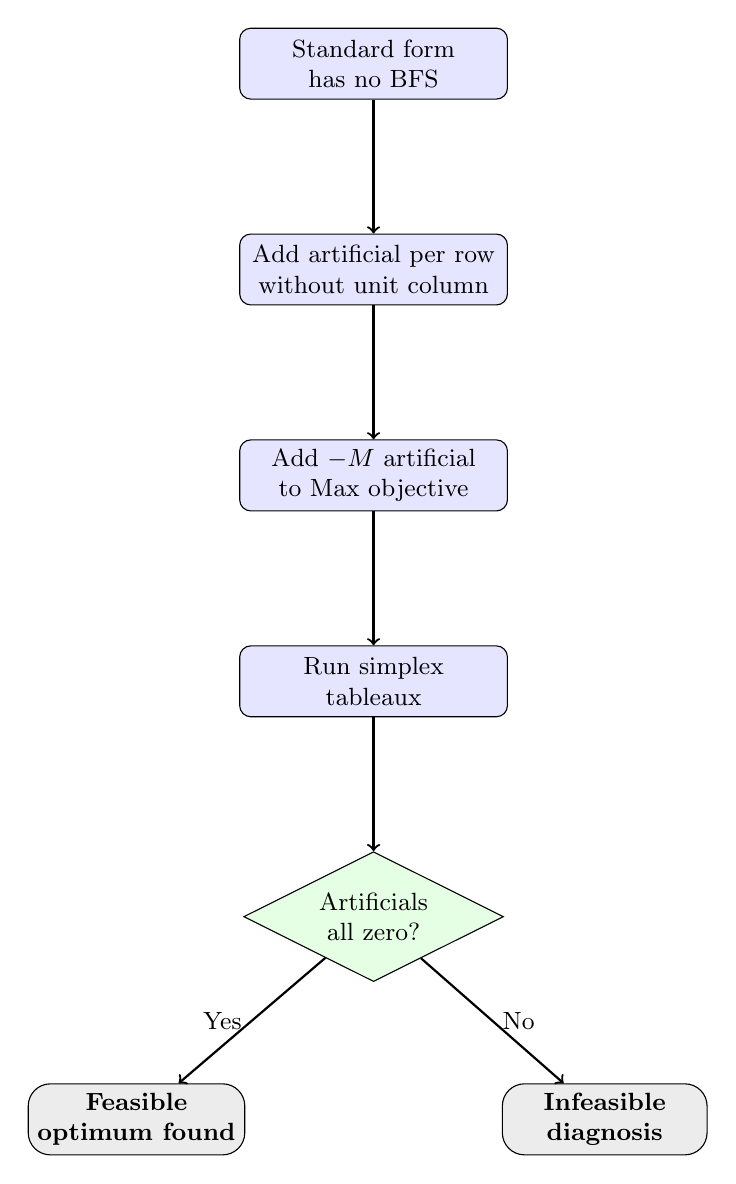
\begin{tikzpicture}[node distance=1.7cm]
\node[proc] (A) {Standard form\\has no BFS};
\node[proc, below=of A] (B) {Add artificial per row\\without unit column};
\node[proc, below=of B] (C) {Add $-M$ artificial\\to Max objective};
\node[proc, below=of C] (D) {Run simplex\\tableaux};
\node[dec, below=of D] (E) {Artificials\\all zero?};
\node[term, below left=1.7cm and 0.8cm of E] (F) {Feasible\\optimum found};
\node[term, below right=1.7cm and 0.8cm of E] (G) {Infeasible\\diagnosis};
\draw[arr] (A) -- (B);
\draw[arr] (B) -- (C);
\draw[arr] (C) -- (D);
\draw[arr] (D) -- (E);
\draw[arr] (E) -- node[left, font=\small] {Yes} (F);
\draw[arr] (E) -- node[right, font=\small] {No} (G);
\end{tikzpicture}
\end{document}
